\documentclass[11pt, letterpaper]{article}

\usepackage[utf8]{inputenc}
\usepackage{graphicx}
\graphicspath{ {images/} }
\usepackage{amsmath}


\title{A First Document}
\author{Mark E. Drummond \thanks{\LaTeX, powered by Overleaf (www.overleaf.com)}}
\date{\today}

\begin{document}

\maketitle

\tableofcontents

\begin{abstract}
    This is a simple paragraph at the beginning of the 
document. A brief introduction about the main subject.
\end{abstract}

https://www.overleaf.com/learn/latex/Learn\_LaTeX\_in\_30\_minutes

\section{Introduction}
 
This is the first section.
 
Lorem  ipsum  dolor  sit  amet,  consectetuer  adipiscing  
elit.   Etiam  lobortisfacilisis sem.  Nullam nec mi et 
neque pharetra sollicitudin.  Praesent imperdietmi nec ante. 
Donec ullamcorper, felis non sodales...
 
\addcontentsline{toc}{section}{Unnumbered Section}
\section*{Unnumbered Section}
 
Lorem ipsum dolor sit amet, consectetuer adipiscing elit.  
Etiam lobortis facilisissem.  Nullam nec mi et neque pharetra 
sollicitudin.  Praesent imperdiet mi necante...
 
\section{Second Section}
 
Lorem ipsum dolor sit amet, consectetuer adipiscing elit.  
Etiam lobortis facilisissem.  Nullam nec mi et neque pharetra 
sollicitudin.  Praesent imperdiet mi necante...

Now that we have written our abstract, we can begin writing our first paragraph.


This line will start a second Paragraph.


We have now added a title, author and date to our first \LaTeX{} document!

Enforced \\
line
\newline
breaks

Some of the \textbf{greatest} discoveries in \underline{science} were made by \textbf{\textit{accident}}.

Some of the greatest \emph{discoveries} in science were made by accident.

\textit{Some of the greatest \emph{discoveries} in science were made by accident.}

\textbf{Some of the greatest \emph{discoveries} in science were made by accident.}

The universe is immense and it seems to be homogeneous, 
in a large scale, everywhere we look at.

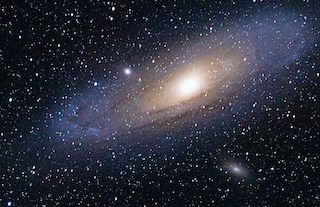
\includegraphics{galaxy}

There's a picture of a galaxy above.

\clearpage

\begin{figure}[h]
    \centering
    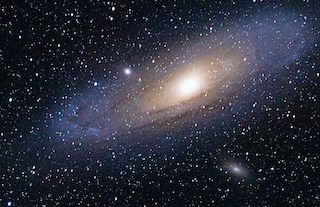
\includegraphics[width=0.25\textwidth]{galaxy}
    \caption{Andromeda}
    \label{fig:andromeda}
\end{figure}

As you can see in the figure \ref{fig:andromeda}, yadda yadda. Also, in the page \pageref{fig:andromeda} is the same example.

% This line here is a comment. It will not be printed in the document.

An unordered list:

\begin{itemize}
    \item This is an item
    \item This is another item
\end{itemize}

An ordered list:

\begin{enumerate}
    \item This is item 1
    \item This is item 2
\end{enumerate}

In physics, the mass-energy equivalence is stated 
by the equation $E=mc^2$, discovered in 1905 by Albert Einstein. Inline math is started and ended with the \$ characters: \$E=mc\textasciicircum{2}\$.

You can also include inline math with \textbackslash( and \textbackslash), or \textbackslash{begin\{math\}} and \textbackslash{end\{math\}}.

The mass-energy equivalence is described by the famous equation (un-numbered display mode):

\[E=mc^2\]

discovered in 1905 by Albert Einstein. In natural units ($c = 1$), the formula expresses the identity (numbered display mode):

\begin{equation}
    E=m
\end{equation}

There's also the $amsmath$ package which provides more math capabilities:

Subscripts in math mode are written as $a_b$ and superscripts are written as $a^b$. These can be combined an nested to write expressions such as
 
$$T^{i_1 i_2 \dots i_p}_{j_1 j_2 \dots j_q} = T(x^{i_1},\dots,x^{i_p},e_{j_1},\dots,e_{j_q})$$
 
We write integrals using $\int$ and fractions using $\frac{a}{b}$. Limits are placed on integrals using superscripts and subscripts:
 
$$\int_0^1 \frac{1}{e^x} =  \frac{e-1}{e}$$
 
Lower case Greek letters are written as $\omega$ $\delta$ etc. while upper case Greek letters are written as $\Omega$ $\Delta$.
 
Mathematical operators are prefixed with a backslash as $\sin(\beta)$, $\cos(\alpha)$, $\log(x)$ etc.

% \part and \chapter are defined in the book and report classes. \part is the highest level of separation. \chapter is next, then the "sections".
%\part{Part 1}
%\chapter{Chapter 1}

\section{Section 1}

\subsection{Sub-section 1}

\subsubsection{Sub-sub-section 1}

\paragraph{Paragraph 1}

\subparagraph{Sub-paragraph 1}

\clearpage

A simple table:

\begin{center}
\begin{tabular}{ c c c }
 cell1 & cell2 & cell3 \\ 
 cell4 & cell5 & cell6 \\  
 cell7 & cell8 & cell9    
\end{tabular}
\end{center}

Check out tablesgenerator.com.

With borders:

\begin{center}
\begin{tabular}{ |c|c|c| } 
 \hline
 cell1 & cell2 & cell3 \\ 
 cell4 & cell5 & cell6 \\ 
 cell7 & cell8 & cell9 \\ 
 \hline
\end{tabular}
\end{center}

\begin{center}
\begin{tabular}{ |l||c|||r| } 
 \hline
 cell1 & cell2 & cell3 \\ 
 \hline
 cell4 & cell5 & cell6 \\ 
 \hline
 \hline
 cell7 & cell8 & cell9 \\ 
 \hline
 \hline
 \hline
\end{tabular}
\end{center}

\begin{center}
 \begin{tabular}{||c c c c||} 
 \hline
 Col1 & Col2 & Col2 & Col3 \\ [0.5ex] 
 \hline\hline
 1 & 6 & 87837 & 787 \\ 
 \hline
 2 & 7 & 78 & 5415 \\
 \hline
 3 & 545 & 778 & 7507 \\
 \hline
 4 & 545 & 18744 & 7560 \\
 \hline
 5 & 88 & 788 & 6344 \\ [1ex] 
 \hline
\end{tabular}
\end{center}

Table references and captions:

Table \ref{table:data} is an example of referenced \LaTeX{} elements.
 
\begin{table}[h!]
\centering
\begin{tabular}{||c c c c||} 
 \hline
 Col1 & Col2 & Col2 & Col3 \\ [0.5ex] 
 \hline\hline
 1 & 6 & 87837 & 787 \\ 
 2 & 7 & 78 & 5415 \\
 3 & 545 & 778 & 7507 \\
 4 & 545 & 18744 & 7560 \\
 5 & 88 & 788 & 6344 \\ [1ex] 
 \hline
\end{tabular}
\caption{Table to test captions and labels}
\label{table:data}
\end{table}


\end{document}